\documentclass[12pt]{article}
\usepackage{graphicx}
\pagestyle{empty}
\setcounter{secnumdepth}{2}

\topmargin=0cm
\oddsidemargin=0cm
\textheight=22.0cm
\textwidth=16cm
\parindent=0cm
\parskip=0.15cm
\topskip=0truecm
\raggedbottom
\abovedisplayskip=3mm
\belowdisplayskip=3mm
\abovedisplayshortskip=0mm
\belowdisplayshortskip=2mm
\normalbaselineskip=12pt
\normalbaselines

\begin{document}

\vspace*{0.5in}
\centerline{\bf\Large Almost Excel}

\vspace*{0.5in}
\centerline{\bf\Large Team 2}

\vspace*{0.5in}
\centerline{\bf\Large 3 January 2013}

\vspace*{1.5in}
\begin{table}[htbp]
\caption{Team}
\begin{center}
\begin{tabular}{|r | c|}
\hline
Name & ID Number \\\hline\hline
Kevin Cameron & 9801448 \\\hline\hline
Addison Rodomista & 1967568 \\\hline\hline
Dragos Dinulescu & 6304826 \\\hline\hline
Adrian Max McCrea & 9801448 \\\hline\hline
Ghazal Zamani & 1971158 \\\hline\hline
Karim Kaidbey & 9654726 \\\hline\hline
Kevin Cameron & 9801448 \\\hline\hline
Kevin Cameron & 9801448 \\\hline\hline
Kevin Cameron & 9801448 \\\hline\hline
Kevin Cameron & 9801448 \\\hline\hline
Kevin Cameron & 9801448 \\\hline\hline
Kevin Cameron & 9801448 \\\hline
\end{tabular}
\end{center}
\end{table}

\clearpage

\section{System}
FunSheets is an electronic spreadsheet program used for storing, organizing and evaluating raw data. FunSheets is designed, written and distributed by Team 2 of COMP354 W/PP

\subsection{Purpose}
FunSheets is used to automate data orginization and the calculations of complex expressions involving large amounts of data.
\subsection{Context}
FunSheets will allow the user to create, open or modify a spread sheet and evaluate the source to produce a new spreadsheet featuring calculated value, evaluated expressions, and sorted information.

\section{Domain Concepts}
\subsection{Domain Model}

\begin{figure}[htbp]
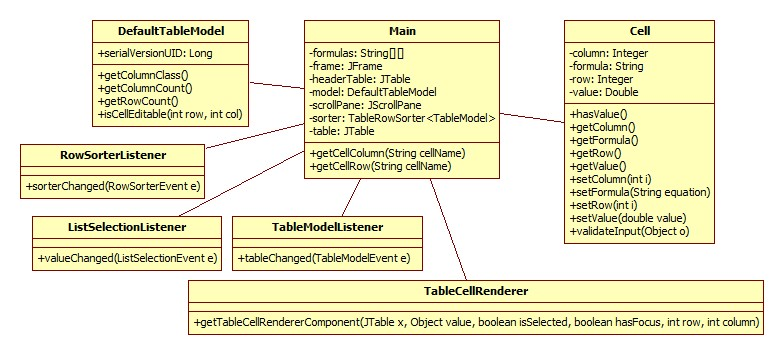
\includegraphics{DomainModel.jpg}
\caption{Domain Model}
\label{fig:Domain-model-diagram}
\end{figure}

\clearpage

\subsection{Main Domain concepts of the users}
\begin{table}[htbp]
\caption{Concepts}
\begin{center}
\begin{tabular}{|r | p{10cm}|}
\hline
Concept & Description \\\hline\hline
Registered Users & A person that has a registered account on funsheets.com can download the software for free and will have access to all future updates \\\hline\hline
Other Users & All other people can download a 30 day trial\\\hline
\end{tabular}
\end{center}
\end{table}

\section{Actors}
A list of actors (primary/secondary), and use cases are mentioned in this section.

\subsection{List of Actors}
\begin{enumerate}
\item Person as a primary actor.
\item System as a secondary actor.
\end{enumerate}

\subsection{Description of Actors}
\begin{enumerate}
\item Person:  A Person, is the main user of the application. Their roll is to input raw data or expressions manually or by opening existing files
\item System:  A software application that provides utilities for spreadsheet analysis and evaluation.
\end{enumerate}

\section{Use Cases}

\subsection{Overview}
Use Case model provides an understanding of the interaction between the user and the software
system. It consists of one or more actors and one or more use cases where actors represent particular
role and use cases represent actions performed by the system. 
\clearpage
\subsection{Use Case Diagram}
\begin{figure}[htbp]
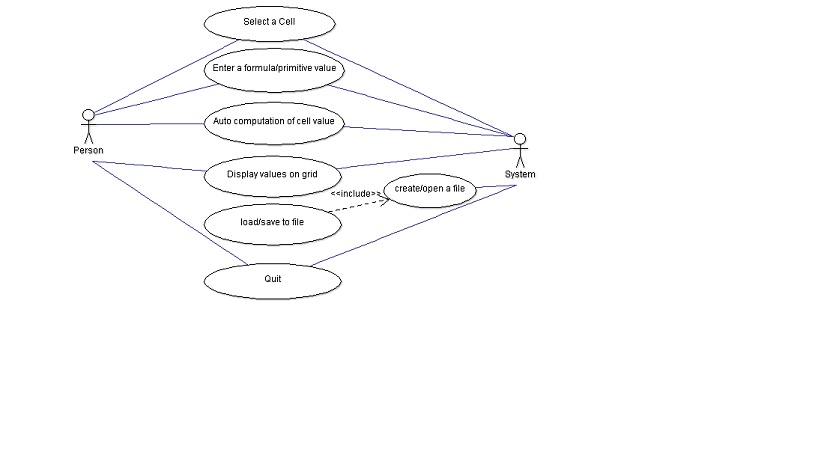
\includegraphics[scale=0.7]{USE_CASE_DIAGRAM.jpg}
\caption{Use Case Diagram}
\label{fig:use-case-diagram}
\end{figure}

\clearpage

\subsubsection{Use Case 1} \label{uc:1}

\noindent
{\bf Name}\\
Select a Cell

\noindent
{\bf Summary}\\
A user will select a cell that can be used for various operations

\noindent
{\bf Actors}\\
1. Person\\
2. System\\

\noindent
{\bf Precondition}\\
The user has opened the program, and opened or created a spread sheet\\
\noindent\\
{\bf Main Scenario}\\
\vspace*{-0.2in}
\begin{enumerate}
\item User will click on the desired cell or enter the cell address.
\end{enumerate}

\noindent
{\bf Exceptions}\\
The cell is outside an acceptable range

\noindent
{\bf Postcondition}\\
Selecting a cell will trigger an event in the system to evaluate the input

\clearpage

\subsubsection{Use Case 2} \label{uc:2}

\noindent
{\bf Name}\\
Enter Formula / Primitive valuel

\noindent
{\bf Summary}\\
The user can enter a primitive value of type real which must have at least
one digit before the decimal point, and if the real number has a decimal part then there is
at least one digit after the decimal point. The numbers may be negative. In addition, the
user can enter a formula which start by equal sign (=) and these formulas are the usual
arithmetic expressions.

\noindent
{\bf Actors}\\
1. Person\\
2. System\\

\noindent
{\bf Precondition}\\
The user has selected a cell\\
\noindent\\

{\bf Main Scenario}\\
\vspace*{-0.2in}
\begin{enumerate}
\item Select a Cell
\item Enter primitive data through standard input devices (eg. keyboard, scanner etc.)
\end{enumerate}

\noindent
{\bf Exceptions}\\
None

\noindent
{\bf Postcondition}\\
Data stored in the selected cell of the spread sheet

\clearpage

\subsubsection{Use Case 3} \label{uc:3}

\noindent
{\bf Name}\\
Automatic Computation

\noindent
{\bf Summary}\\
When a cell contains an expression the system will parse the string and evaluate the elements to produce a value.

\noindent
{\bf Actors}\\
1. System\\

\noindent
{\bf Precondition}\\
A cell contains an expression\\
\noindent\\
{\bf Main Scenario}\\
\vspace*{-0.2in}
\begin{enumerate}
\item User opens the program
\item User enters an expression, or loads a sheet with expressions
\item The user selects Automatic computation
\end{enumerate}

\noindent
{\bf Exceptions}\\
None

\noindent
{\bf Postcondition}\\
The cell that contains the expression will display the results of the evaluation

\clearpage

\subsubsection{Use Case 4} \label{uc:4}

\noindent
{\bf Name}\\
Display On Screen

\noindent
{\bf Summary}\\
Output the spreadsheet as a grid of cells with values and evaluated expressions.

\noindent\\
{\bf Actors}\\
1. System\\

\noindent
{\bf Precondition}\\
Program is open\\
A spreadsheet has been created or loaded\\
\noindent\\
{\bf Main Scenario}\\
\vspace*{-0.2in}
\begin{enumerate}
\item User opens the program
\item User enters an expression, or loads a sheet with expressions
\item System will display the results in a grid of cells.
\end{enumerate}

\noindent
{\bf Exceptions}\\
None

\noindent\\
{\bf Postcondition}\\
A GUI representation of the grid is displayed with evalutated cells in a row / column grid.

\clearpage


\subsubsection{Use Case 5} \label{uc:5}

\noindent
{\bf Name}\\
File management

\noindent
{\bf Summary}\\
Allow the user to load or save an existing spreadsheet to disk

\noindent
{\bf Actors}\\
1. System\\
2. User \\

\noindent
{\bf Precondition}\\
Program is open\\
\noindent\\
{\bf Main Scenario}\\
\vspace*{-0.2in}
\begin{enumerate}
\item User opens the program
\item User loads an existing file
\item User can make modifications to the spreadsheet
\item System will evaluate the results
\item User save the changes to disk
\end{enumerate}

\noindent
{\bf Exceptions}\\
None

\noindent
{\bf Postcondition}\\
A GUI representation of the grid is displayed with evalutated cells in a row / column grid.

\clearpage

\section{Non-Functional Constraints}

\begin{tabular}{| l | l | p{3cm} | l | p{3cm} | l | p{3cm} |}
\hline
ID&Ver&Requirement&Source&Rationale&Status&Traces to use case\\\hline
No.1 & 1 & User must be registered & IT manager & access information about the users&implemented&Register, login, download\\\hline

\end{tabular}

\section{Data Dictionary}

\section{References}

\appendix

\section{Description of File Format: Input}
\noindent\\
The application accepts a .CSV file (Comma seperated value).  A CSV file consists of any number of records, separated by line breaks of some kind. The line break represent the start of a new row of data. Each Row consists of fields, separated by some other character or string, most commonly a literal comma ( , ) or tab. Usually, all records have an identical sequence of fields.

\section{Description of File Format: Output}
\noindent\\
{\bf Display Output}: \\The display output is a grid of cells that are arranged into rows and columns. Each cells that contain primitive data are displayed without modification to their contents. Cells that contain expressions are displayed with their expressions evaluated into usable data.
\noindent\\\\
{\bf File Output}:\\When a spreadsheet is saved each cell is converted to a field and exported to a CSV file. Cells that contain primitive values will be exported without modification. Cells that contain expressions will be exported as a string representation of the expression.\\

\end{document}
